\chapter[Modelos de regresi\'on]{Modelos de regresi\'on}

\section{Concepto general}

Los modelos de regresi\'on tienen como objetivo describir la distribuci\'on de una variable aleatoria $y \in \mathbb{R}$, generalmente llamada \textit{variable de respuesta}, condicional a los valores de las variables $x \in \mathbb{R}^n$, conocidas como \textit{covariables}, \textit{variables explicativas} o \textit{variables predictivas}. Visto en t\'erminos matem\'aticos, se puede expresar como
\begin{equation*}
    y|x \sim \mathbb{P}(y|x).
\end{equation*}

Si bien esta relaci\'on se da por hecha y se supone un v\'inculo concreto del que provinieron los datos, normalmente dicho v\'inculo es desconocido. Por lo tanto, la intenci\'on de estos modelos es realizar alguna estimaci\'on de \'el. Dado que es complicado aproximar con exactitud toda la distribuci\'on, com\'unmente se utilizan un n\'umero finito de par\'ametros para describirla. Adem\'as, la interpretaci\'on de dichos par\'ametros suele tener relevancia para el modelador, como es el caso de la media o la mediana. 

Tambi\'en es importante resaltar que este trabajo tiene inter\'es en modelar a $y$, dado que ya se observaron los valores de $x$. Sin embargo, se podr\'ia pensar en modelos donde tenga sentido la distribuci\'on conjunta de $y$ y $x$, misma que se podr\'ia obtener como
\begin{equation*}
    \mathbb{P}(y,x) = \mathbb{P}(y|x) \times \mathbb{P}(x).
\end{equation*}

\section{Regresión a la media}

La \textit{regresi\'on a la media} es el caso particular m\'as usado de los modelos de regresi\'on, tanto en el paradigma Bayesiano, como en otros. Esto sucede debido al bajo uso de recursos que requiere su estimaci\'on. En el caso particular Bayesiano, familias conjugadas tienen sentido dentro de este contexto, y en otros paradigmas suelen ser usados debido a que se asocian con la minimizaci\'on de t\'erminos cuadrados, con las bondades de diferenciabilidad que eso implica. Adem\'as, cuando se supone una relaci\'on param\'etrica entre la variable de respuesta y las covariables, se valora la capacidad interpretativa que tienen los par\'ametros estimados.

En notaci\'on probabil\'istica, retomando el hecho de que $y|x \sim \mathbb{P}(y|x)$, el modelo de regresi\'on a la media busca aproximar a la funci\'on $f$, tal que 
\begin{equation*}
    \mathbb{E}[y|x] = f(x).
\end{equation*}
Para hacer esto, normalmente se vale del supuesto que
\begin{equation*}
    y = f(x) + \varepsilon,
\end{equation*}
con $\varepsilon \in \mathbb{R}$ (denominado com\'unmente como el \textit{error aleatorio}), una variable aleatoria independiente de $x$, tal que $\mathbb{E}[\varepsilon] = 0$. Adem\'as, $f: \mathbb{R}^n \rightarrow \mathbb{R}$ es desconocida, pero fija. As\'i, debido a que la esperanza de la suma es la suma de las esperanzas, se cumple que $\mathbb{E}[y|x] = f(x)$.

Adem\'as, se supone independencia entre los errores. Por lo tanto, sean $\tilde{x}$ las covariables asociadas a la variable de respuesta $\tilde{y}$, y $\dot{x}$ las asociadas a $\dot{y}$, se tiene que $\tilde{y} | \tilde{x}, f$ es condicionalmente independiente a $\dot{y} | \dot{x}, f$.

\subsection[Modelo tradicional]{
    Modelo tradicional
    \footnote{Algunas ideas de esta subsecci\'on son retomadas de \cite{Denison_BayesMethods} y \cite{Bannerjee_BayLinMod}.}
}

La \textit{regresi\'on lineal a la media} es el caso particular m\'as usado en el contexto de regresi\'on a la media. Consiste en definir
\begin{equation*}
    f(x) = x^T\beta,
\end{equation*}
donde $\beta \in \mathbb{R}^n$ se piensa con valores constantes, pero desconocidos, y la tarea es estimarlos. Adem\'as, se supone error normal, es decir, $\varepsilon \sim \mathcal{N}(0,\sigma^2)$, tal que el par\'ametro de varianza fijo $\sigma^2$ tambi\'en debe ser estimado.

Para hacer esto, el enfoque Bayesiano le asigna una distribución inicial de probabilidad a ambos par\'ametros, reflejando la incertidumbre que tiene el modelador acerca de su valor real. Es decir, se tiene que 
\begin{equation*}
    \beta,\sigma^2 \sim \mathbb{P}(\beta,\sigma^2).
\end{equation*}

Sea $\{(x_i,y_i)| x_i \in \mathbb{R}^n, y_i \in \mathbb{R}, i \in \{1,...,m\} \}$ el conjunto de datos observados de las variables de respuesta y de las covariables. Es posible representar este mismo conjunto con la notaci\'on matricial $\{X,Y | X \in \mathbb{R}^{m \times n}, Y \in \mathbb{R}^m\}$. \footnote{Por simplificaci\'on y limpieza de notaci\'on en este trabajo se escribir\'an de igual manera variables aleatorias y los datos en efecto observados, considerando que en cada caso el contexto ser\'a suficiente para saber de cu\'al se est\'a hablando, siendo asociadas las letras min\'usculas a una \'unica observaci\'on y las may\'usuclas a una matriz de observaciones.} Sea $\mathcal{E} \in \mathbb{R}^m$ el vector de errores aleatorios, tal que $\mathcal{E} \sim \mathcal{N}(0,\sigma^2 I)$. El modelo se puede reescribir como:
\begin{equation*}
\begin{aligned}
    Y &= X\beta + \mathcal{E}, \\
    Y|X,\beta,\sigma^2 &\sim \mathcal{N}(X\beta,\sigma^2 I).
\end{aligned}
\end{equation*}

De esta manera, se tiene una distribuci\'on para la variable aleatoria $Y$, dada $X$, que para poder ser expresada, requiere de la estimaci\'on de $\beta$ y $\sigma^2$. Dicha estimaci\'on la hace partiendo de la aproximaci\'on de la media te\'orica, utilizando los datos observados y los supuestos antes mencionados.

Por el Teorema de Bayes,
\begin{equation*}
\begin{aligned}
    \mathbb{P}(\beta,\sigma^2 | Y, X) 
    &= \frac{\mathbb{P}(Y| X, \beta, \sigma^2) \times \mathbb{P}(\beta, \sigma^2 | X)}{P(Y | X)} \\
    &= \frac{\mathbb{P}(Y| X, \beta, \sigma^2) \times \mathbb{P}(\beta, \sigma^2)}{\mathbb{P}(Y | X)} \\
    &\propto \mathbb{P}(Y| X, \beta, \sigma^2) \times \mathbb{P}(\beta, \sigma^2), \\
\end{aligned}
\end{equation*}
donde $\mathbb{P}(Y| X, \beta, \sigma^2)$ es la verosimilitud de los datos observados y, debido a la independencia condicional, se puede calcular como $\mathbb{P}(Y| X, \beta, \sigma^2) = \mathcal{N}(X\beta,\sigma^2 I) = \prod_{i=1}^m \mathcal{N}(x_i^T\beta,\sigma^2)$. 

Por conveniencia anal\'itica, hay una distribuci\'on inicial com\'unmente usada para los par\'ametros $\beta$ y $\sigma$ debido a que es conjugada respecto a la distribuci\'on Normal de los datos. Su nombre es \textit{Normal-Gamma Inversa (NGI)} y se dice que $\beta,\sigma^2 \sim \mathcal{NGI}(M,V,a,b)$, si
\begin{equation*}
\begin{aligned}
    \mathbb{P}(\beta,\sigma^2) 
    &= \mathbb{P}(\beta|\sigma^2) \times \mathbb{P}(\sigma^2) \\
    &= \mathcal{N}(\beta|M, \sigma^2 V) \times \mathcal{GI}(\sigma ^2|a,b) \\
    &\propto (\sigma^2)^{-(a+(n/2)+1)} \exp\left(-\frac{(\beta-M)^TV^{-1}(\beta-M) + 2b}{2\sigma^2}\right),
\end{aligned}
\end{equation*}
donde $M$ es la media inicial de los coeficientes, $\sigma^2 V$ la matriz de varianzas y covarianzas, y $a$, $b$ son los par\'ametros iniciales de forma y escala, respectivamente, de $\sigma ^2$. 

Aprovechando la propiedad conjugada, es posible escribir la densidad posterior de los par\'ametros como
\begin{equation*}
\begin{aligned}
    \mathbb{P}(\beta,\sigma^2 | Y, X) 
    &\propto \mathbb{P}(Y| X, \beta, \sigma^2) \times \mathbb{P}(\beta, \sigma^2), \\
    &\propto (\sigma^2)^{-(\bar{a}+(n/2)+1)} \exp\left(-\frac{(\beta-\bar{M})^T\bar{V}^{-1}(\beta-\bar{M}) + 2\bar{b}}{2\sigma^2}\right),
\end{aligned}
\end{equation*}
donde
\begin{equation*}
\begin{aligned}
    \bar{M} &= (V^{-1} + X^TX)^{-1} (V^{-1}M + X^TY), \\
    \bar{V} &= (V^{-1} + X^TX)^{-1}, \\
    \bar{a} &= a + n/2, \\
    \bar{b} &= b + \frac{\bar{M}^TV^{-1}M + Y^TY - \bar{M}^T\bar{V}^{-1}\bar{M}}{2}.
\end{aligned}
\end{equation*}

Es decir, la distribuci\'on posterior de $(\beta,\sigma^2)$ es \textit{Normal - Gamma Inversa}, con par\'ametros $\mathcal{NGI}(\bar{M},\bar{V},\bar{a},\bar{b})$.

Si se tiene una nueva matriz de covariables $X_*$ y se desea hacer predicci\'on de las respectivas variables de salida $Y_*$, es posible hacer inferencia con los datos observados como se detalla a continuaci\'on.
\begin{equation*}
\begin{aligned}
    \mathbb{P}(Y_*|X_*,Y,X)
    &= \int \int \mathbb{P}(Y_*|X_*,\beta,\sigma^2) \times \mathbb{P}(\beta,\sigma^2|Y,X) d\sigma^2 d\beta \\
    &= \int \int \mathcal{N}(Y_*|X_*\beta,\sigma^2I) \times \mathbb{P}(\beta,\sigma^2|Y,X) d\sigma^2 d\beta.
\end{aligned}
\end{equation*}

Particularmente, si se contin\'ua con el modelo conjugado \textit{Normal - Gamma Inversa / Normal}, es posible encontrar la soluci\'on anal\'itica:
\begin{equation*}
\begin{aligned}
    \mathbb{P}(Y_*|X_*,Y,X)
    &= \int \int \mathcal{N}(Y_*|X_*\beta,\sigma^2I) \times \mathcal{NGI}(\beta,\sigma^2|\bar{M},\bar{V},\bar{a},\bar{b}) d\sigma^2 d\beta \\
    &= MVSt_{2\bar{a}} 
       \left(
        X_*\bar{M},\frac{\bar{b}}{\bar{a}}\left(I + X_*\bar{V}X_*^T\right)
       \right),
\end{aligned}
\end{equation*}
donde $MVSt$ es la distribuci\'on \textit{t-Student} multivariada, y cuya definici\'on se describe en el \autoref{chap:Distributions}.

\section{Regresión sobre cuantiles}

La \textit{regresi\'on sobre cuantiles} es una alternativa que se ha desarrollado reci\'entemente y que permite enfocarse en aspectos alternativos de la distribuci\'on, por ejemplo, lo que pasa en las colas o en alg\'un decil de inter\'es. 

\begin{defin}
Sea $F_y$ la funci\'on de distribuci\'on de la variable aleatoria $y$, entonces la funci\'on que regresa su cuantil p-\'esimo se escribe
\begin{equation*}
    q_p(y)\,=\,\inf \left\{x\in {\mathbb  {R}}:p\leq F_y(x)\right\};
\end{equation*}
que se puede simplificar a
\begin{equation*}
    q_p(y)=F_y^{-1}(p),
\end{equation*}
cuando $F_y$ es continua y estrictamente creciente en el soporte de $y$.
\end{defin}
Dicho en otras palabras, si se tiene un conjunto grande de realizaciones de una variable aleatoria $y$, se esperar\'a que el $p \times 100\%$ est\'e por debajo de $q_p(y)$ y el $(1-p) \times 100\%$ est\'e por arriba. Por ejemplo, la mediana es un caso particular de un cuantil, espec\'ificamente el $0.5$-\'esimo. 

En notaci\'on probabil\'istica, se buscar\'a aproximar a la funci\'on $f$, tal que 
\begin{equation*}
    q_p(y|x) = f(x),
\end{equation*}
para $p \in (0,1)$ arbitrario y fijo.

Para hacer esto, normalmente se valdr\'a del supuesto que
\begin{equation*}
    y = f_p(x) + \varepsilon_p,
\end{equation*}
con $\varepsilon_p \in \mathbb{R}$, una variable aleatoria tal que $q_p(\varepsilon_p) = 0$. Asimismo, $f_p: \mathbb{R}^n \rightarrow \mathbb{R}$ es desconocida, pero fija. Por ello, debido a que el cuantil de una suma es la suma de los cuantiles, se cumple que $q_p(y|x) = f(x)$.

Al igual que con la regresi\'on a la media, se supone independencia entre los errores, y, por lo tanto, hay independencia condicional entre las observaciones.

\subsection{Modelo tradicional}

Cuando surgi\'o entre la comunidad estad\'istica el problema de \textit{regresi\'on sobre cuantiles} inicialmente fue modelado bajo un enfoque no Bayesiano, como se describe en \cite{Yu_BayQuantReg}.  Posteriormente, Koenker \& Bassett (1978) retomaron esas ideas, y las aplicaron en el paradigma Bayesiano. 

Al igual que en la regresi\'on a la media, el primer y m\'as popular modelo ha sido el lineal. Es decir, para $p \in (0,1)$ fijo arbitrario, se define
\begin{equation*}
    f_p(x) = x^T\beta_p, 
\end{equation*}
donde $\beta_p$ es el vector de coeficientes, dependiente de $p$.

\begin{defin}
    Se define a la funci\'on
    \begin{equation*}
    \begin{aligned}
        \rho_p(u) = u \times [pI_{(u>0)} - (1-p) I_{(u<0)})]
        =
        \begin{cases}
            up &\text{ si } u\geq0 \\
            -u(1-p) &\text{ si } u<0 \\
        \end{cases}
        .
    \end{aligned}
    \end{equation*}

    Se dice que una variable aleatoria u sigue una distribuci\'on asim\'etrica de Laplace ($u \sim AL_p(\sigma)$) si su funci\'on de densidad se escribe como
    \begin{equation*}
        w_p^{AL}(u|\sigma) = 
        \frac{p(1-p)}{\sigma}
        exp\left[
        -\rho_p
        \left(
        \frac{u}{\sigma}
        \right)
        \right],
    \end{equation*}
con $p$ par\'ametro de asimetr\'ia y $\sigma$, de escala.
\end{defin}

Para entender mejor las propiedades de dicha distribuci\'on, se presentan las siguientes gr\'aficas.

\begin{figure}[H]
	\centering
	\caption{Funci\'on de densidad de la distribuci\'on asim\'etrica de Laplace, con $\sigma = 1$ y $p$ variable.}
	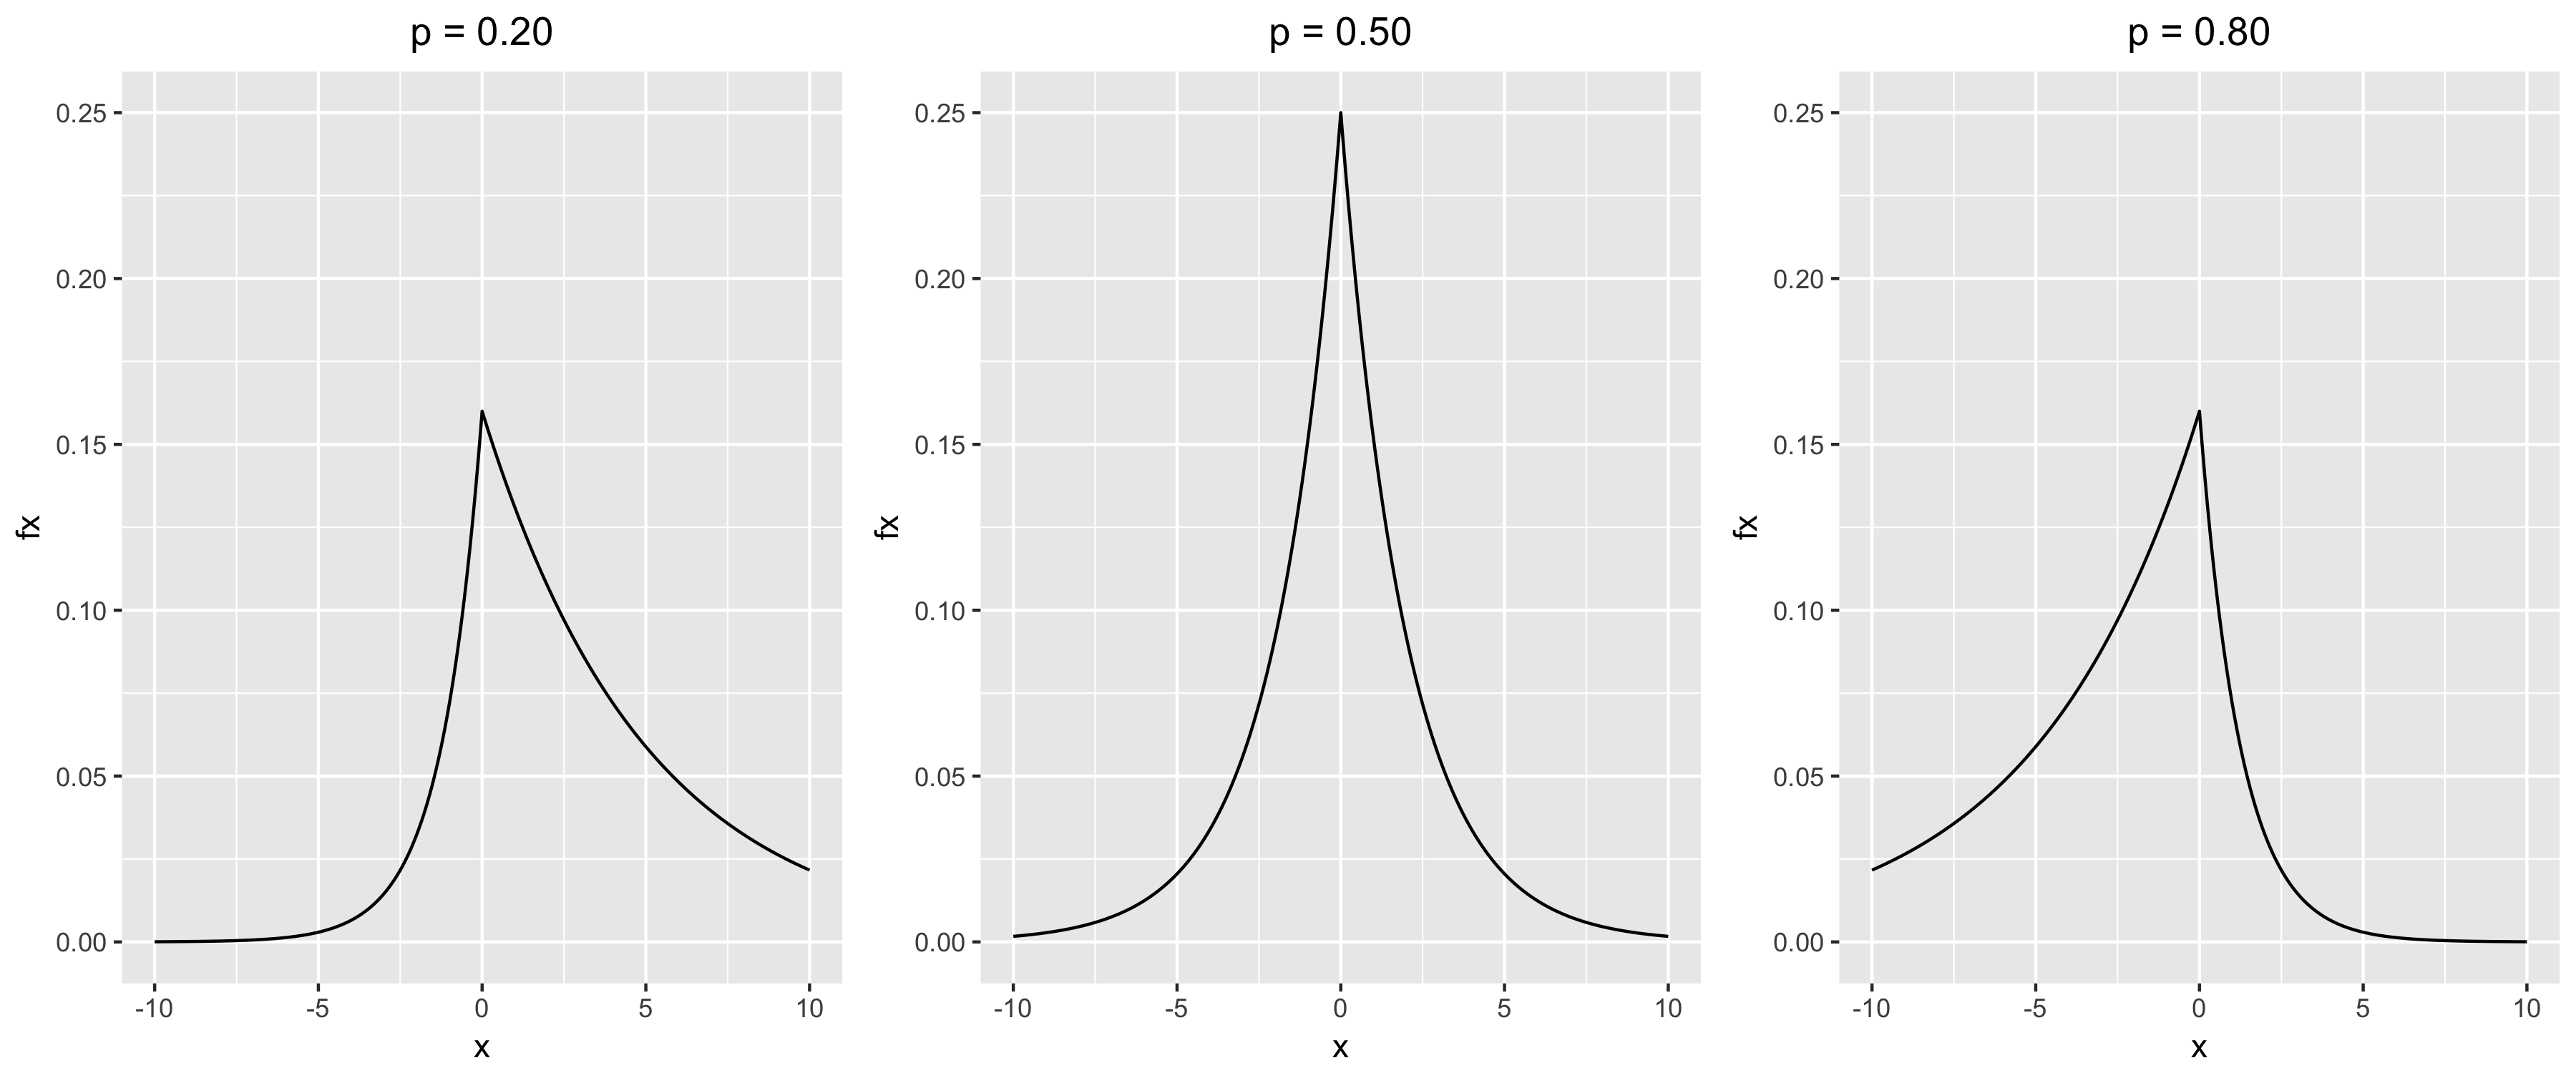
\includegraphics[width=1\textwidth]{Figures/ALD/p_plots.png}
	\label{p_plots}
\end{figure}

\begin{figure}[H]
	\centering
	\caption{Funci\'on de densidad de la distribuci\'on asim\'etrica de Laplace, con $p = 0.25$ y $\sigma$ variable.}
	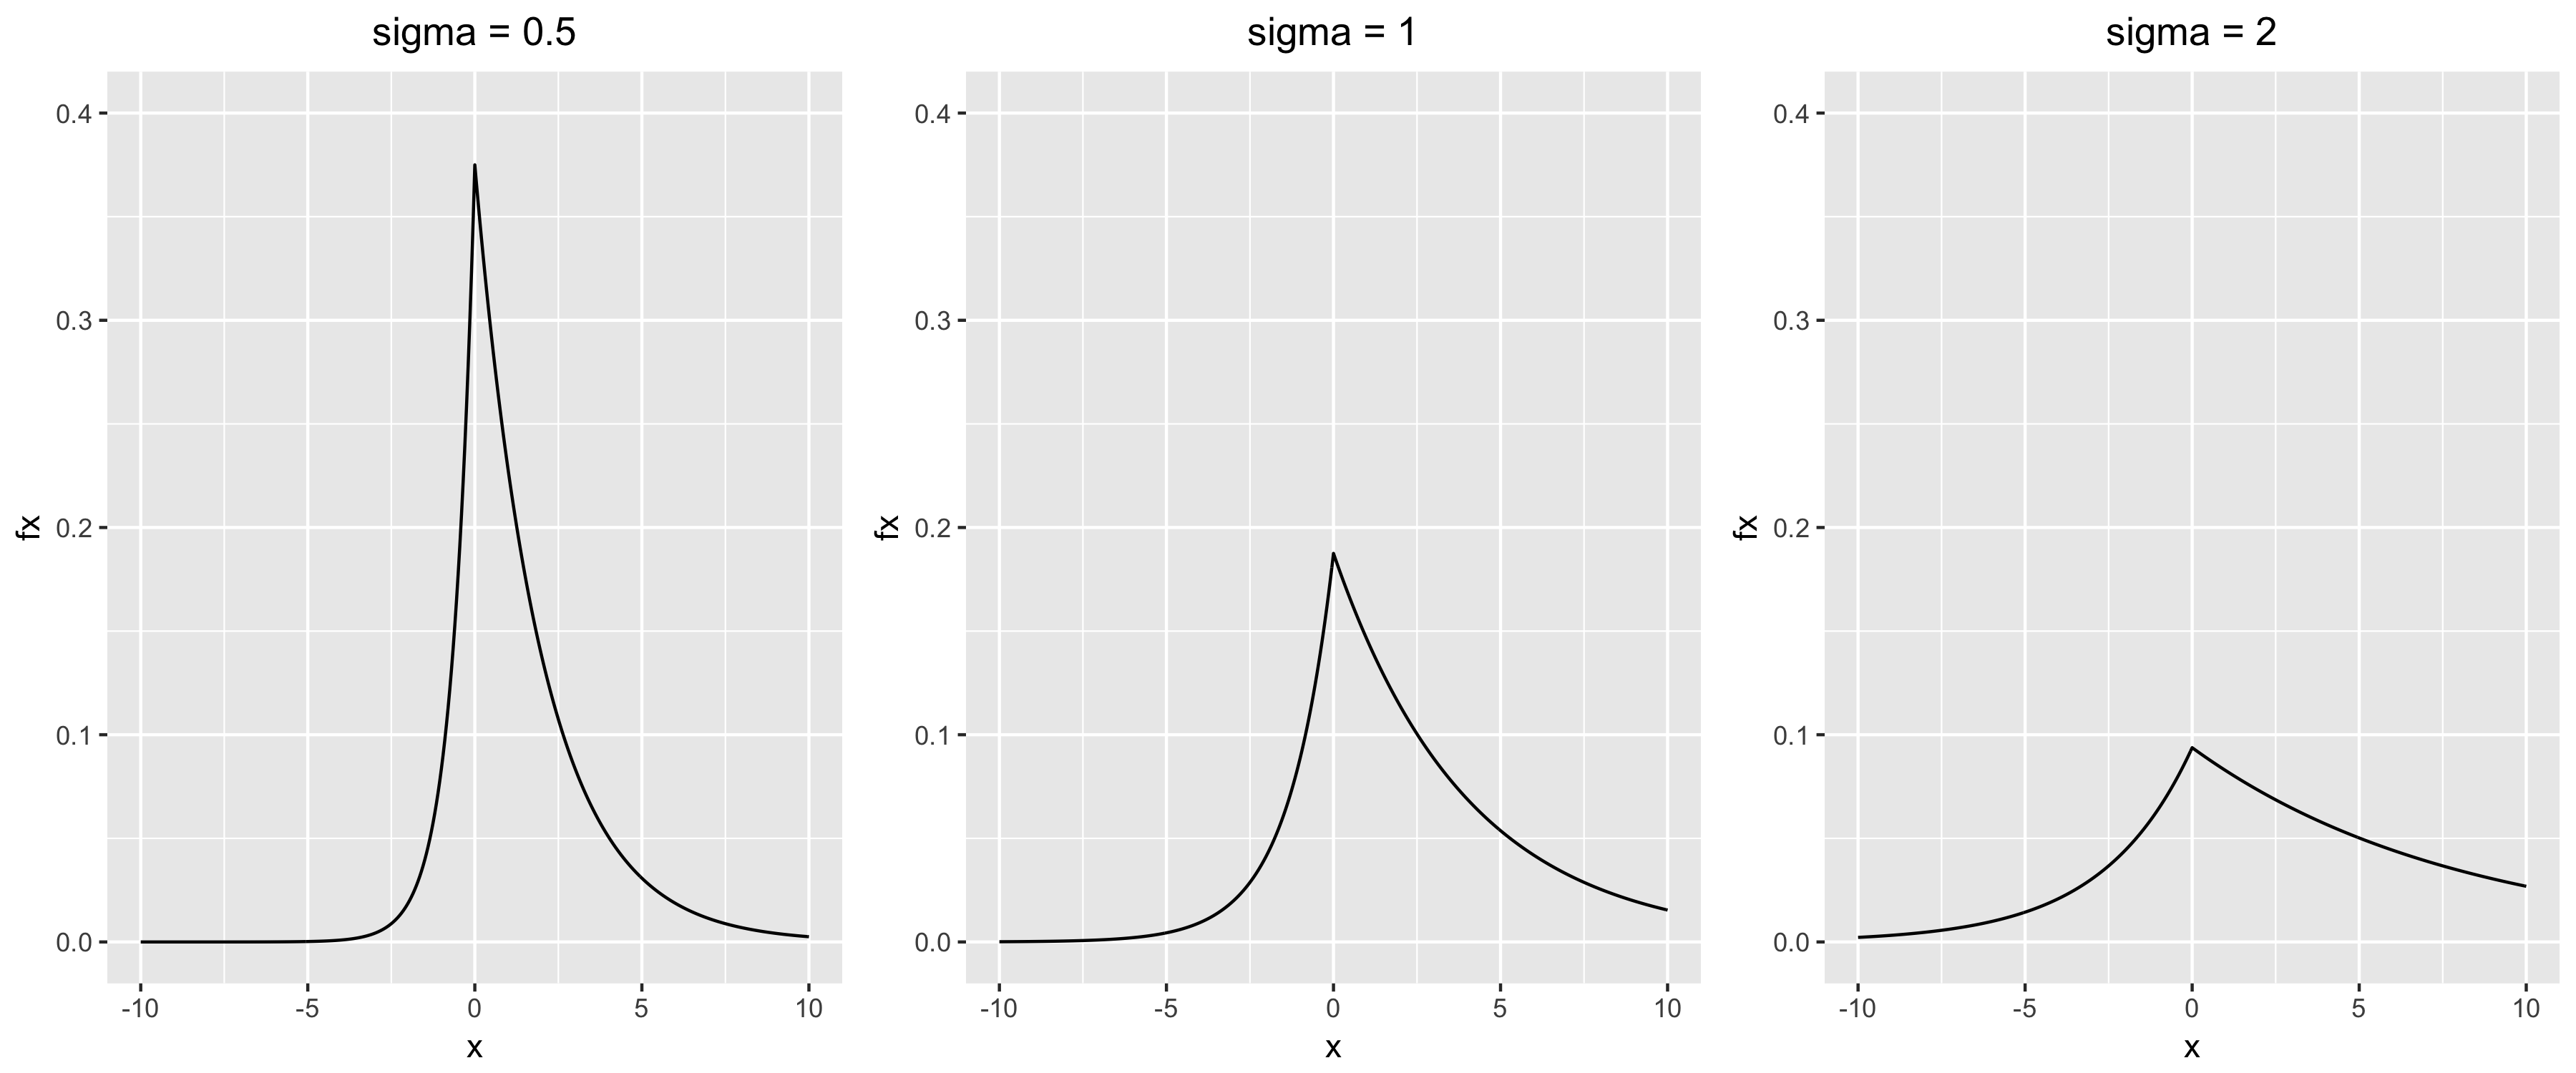
\includegraphics[width=1\textwidth]{Figures/ALD/sigma_plots.png}
	\label{p_plots}
\end{figure}

Como se puede observar, el par\'ametro $p$ representa la asimetr\'ia de la distribuci\'on. Para valores por debajo de $0.5$, la distribuci\'on est\'a sesgada a la derecha, mientras que para valores superiores a $0.5$, presenta sesgo a la izquierda. El \'unico caso en el que es sim\'etrica, es cuando $p = 0.5$. 

Por otro lado, el par\'ametro $\sigma$ representa la dispersi\'on de la distribuci\'on. A menor $\sigma$, los datos, aunque sesgados, estar\'an m\'as concentrados; en cambio, conforme crezca $\sigma$, la cola de la distribuci\'on ser\'a m\'as pesada.

Dicho esto, la propiedad m\'as relevante para este trabajo, es que se puede demostrar que si $\varepsilon_p \sim AL_p(\sigma)$, entonces $q_p(\varepsilon_p) = 0$, independientemente del valor de $\sigma$. Recordando que esa es la \'unica caracter\'istica que pide el modelo general, el modelo tradicional utiliza esta distribuci\'on para explicar la dispersi\'on del error.

Es posible, entonces, reescribir el modelo como
\begin{equation*}
    y | x, \beta_p, \sigma 
    \sim 
    AL_p(y - x^T\beta_p|\sigma).
\end{equation*}

De nueva cuenta, se tiene una distribuci\'on para la variable aleatoria $Y$, dada $X$. En este caso, para poder expresarla requiere de la estimaci\'on de $\beta_p$ y $\sigma$. Dicha estimaci\'on la hace partiendo de la aproximaci\'on del $p-$\'esimo cuantil te\'orico, utilizando los datos observados y los supuestos antes mencionados.

Sea $\{(X,Y) | X \in \mathbb{R}^{m \times n}, Y \in \mathbb{R}^m\}$ el conjunto de datos observados. Por el Teorema de Bayes,
\begin{equation*}
\begin{aligned}
    \mathbb{P}(\beta_p,\sigma | Y, X) 
    &\propto \mathbb{P}(Y| X, \beta_p, \sigma) \times \mathbb{P}(\beta_p, \sigma), \\
\end{aligned}
\end{equation*}
donde $\mathbb{P}(Y| X, \beta_p, \sigma)$ es la verosimilitud, y debido a la independencia condicional, se puede calcular como 
\begin{equation*}
    \mathbb{P}(Y| X, \beta_p, \sigma)
    =
    \prod_{i=1}^m AL_p(y_i - x_i^T\beta_p|\sigma).
\end{equation*}

Por otro lado, $\mathbb{P}(\beta_p,\sigma^2)$ es la distribuci\'on inicial de los par\'ametros, para los que normalmente se usa
\begin{equation*}
    \beta_p,\sigma \sim \mathcal{NGI}(M,V,a,b). 
\end{equation*}

A diferencia del modelo tradicional de regresi\'on a la media, este modelo no es conjugado. Por lo tanto se requieren m\'etodos computacionales (como los que ser\'an descritos en el cap\'itulo 5) para aproximar la distribuci\'on posterior.

En el caso de la predicci\'on, si se tiene una nueva matriz de covariables $X_* \in \mathbb{R}^{r \times n}$, la inferencia con los datos observados se realiza de la siguiente manera:
\begin{equation*}
\begin{aligned}
    \mathbb{P}(Y_*|X_*,Y,X)
    &= \int \int \mathbb{P}(Y_*|X_*,\beta_p,\sigma) \times \mathbb{P}(\beta_p,\sigma|Y,X) d\sigma d\beta_p \\
    &= \int \int \prod_{i=1}^r AL_p(y_{i*} - x_{i*}^T\beta_p|\sigma) \times \mathbb{P}(\beta_p,\sigma|Y,X) d\sigma d\beta_p,
\end{aligned}
\end{equation*}
que tampoco tiene expresi\'on anal\'itica simplificada.

Si bien este modelo representa una buena alternativa, a\'un queda la posibilidad de retomar estas ideas y crear modelos m\'as flexibles, que capturen con mayor precisi\'on las particularidades de cada fen\'omeno y la interacci\'on entre las variables de salida y las covariables. En el siguiente cap\'itulo se discutir\'a la importancia de capturar mayor complejidad en la distribuciones mediante el de uso de m\'etodos no param\'etricos.